\chapabstract{
This appendix highlights the packaging approach, recipes, and procedures developed to interface with photonic integrated circuits within the Princeton University's Lightwave Lab from 2017 to 2023. \\ \textbf{Authors: Eric C. Blow, Bert Harrop, Simon Bilodeau, Thomas Ferreira de Lima} 
}
\section{Introduction}

\qquad Packaging, whilst often overlooked, plays a critical role in the overall performance of integrated circuits. A next-generation processor requires equally state-of-the-art interfacing or performance is unnecessarily degraded. PICs enable ultra-wide instantaneous bandwidths of 10 GHz and frequency tunability from MHz to 100 GHz. This unprecedented bandwidth performance generates a novel electrical interfacing requirement \cite{PIC_Packaging1,PIC_Packaging2_ePIX}. Historically in the Lightwave Laboratory, RF electrical I/O on PICs were probed, while this is sufficient for low number of I/O ($\leq 6$; 3 sides of GSGSG RF probes) and for lab bench experiments, the technique does not support commercialization or growing chip complexities. A fully packaged solution increased functionality through interfacing with co-packaged CMOS and control electronics.

\qquad Traditional wirebonding techniques can support high-speed connections up to 100 GHz. This performance is achieved by keeping wirebond lengths short and pairing the bonds with impedance-matched transmission lines, resulting in narrowband gain at the operating frequency. Wedge wire bonding can be optimized to achieve 30 GHz instantaneous bandwidth (IBW), strip wire bonding can increase IBW to 50 GHz, but beyond that requires the transition to flip-chip bonding \cite{PIC_Packaging3_100GHz,PIC_Packaging4_100GHz2}. 

\qquad In addition to the bandwidth consideration of electrical packaging PICS, the growing complexity of neuromorphic PICs required an increase in the amount and density of electrical I/O. Immediately after demonstrations of a small PNN with 2 neurons, the size of the PNN was limited due to packaging. Electrical probing limited the electrical I/O to 48 connections (16 DC probes over 3 sides of the PIC, 1 side reserved for optical I/O). A simple approximation for electrical I/O required is shown in eqn. /ref{eqn:IOcount}. Two connections, ground and signal, per weight and neuron bias. For an all-to-all connected PNN, the number of weights scale with the number of neurons squared, and lastly each neuron requires a bias. Therefore, probing could only support a PNN with four neurons. 

\begin{equation}
    Number of I/O = 2[Weights + Neuron Bias] = 2[(Neurons^2) + Neurons].
    \label{eqn:IOcount}
\end{equation}

\qquad Transitioning from probing to wedge wire bonding, scales available I/O from number of 3*probe size to a function of the perimeter length and therefore enables larger networks. For an electrical pad of width 100$\mu m$ and a pitch of 150$\mu m$, a standard 3$mm$ by 6$mm$ PIC size could support 100 electrical I/O and therefore a PNN size of 6. With perimeter wire bonding, multiple rows can be implemented if they are interlaced and separated by height. We developed a three-row recipe that increased the electrical I/O count to 300 and therefore a PNN size of 11. Multiplexing signals and common grounds could increase the number of neurons by a few. However, to exceed this number requires using the entire chip surface for electrical I/O instead of simply the perimeter. The PNN complexity scales with the area of the chip, but the electrical I/O with wire bonding scales with the perimeter. The discrepancy in these scaling laws leads to inefficiencies. Therefore, to increase the size of PNNs further requires the transition to flip-chip bonding or co-integrated CMOS control.

\qquad During this , the Lightwave Laboratory transitioned our packaging approach from probing PICs to a fully wire-bonded approach which supports 20 GHz RF connections, 300 of DC control I/O, and epoxied optical coupling. 

\section{Packaging Approach}
(Refer to Chapter 7: Silicon MPC for a detailed example)

\qquad Figure \ref{FigAppA1} below summarizes the packaging approach for interfacing with the silicon microwave photonic canceller (MPC). The goals of the packaging approach were to have RF and DC electrical interfaces with two cancellers on-chip simultaneously. Physically secure the chip in a planar orientation while having sidewall access for optical edge coupling. Lastly, PICs require temperature control. 

\qquad The MPC PIC has 45 electrical DC connections for two separate cancellers, 2 RF outputs which support DC-GSG-DC probes, and 2 RF inputs which support GSGSG probes. The on-chip electrical DC pad array consists of two rows of 23 and 22 aluminum pads, 100$\mu m$ wide by 200$\mu m$ long, pitched 150$\mu m$. The MPC PIC has 19 relevant optical edge couplers but only requires a maximum of 10 to be interfaced simultaneously. 

\qquad The MPC PIC is first interfaced with a custom-fabricated glass expander with an identical DC pad array to that which is on the PIC. This helps to keep the wire bonds as short as possible and parallel to one another. The expander pad array is then fanned out to a lower density single row pad array. This array is matched to a custom-made chip carrier which can be soldered to a printed circuit board. The chip carrier is then diced on one side in order to support optical edge coupling. 

\begin{figure}[!ht]
\centering
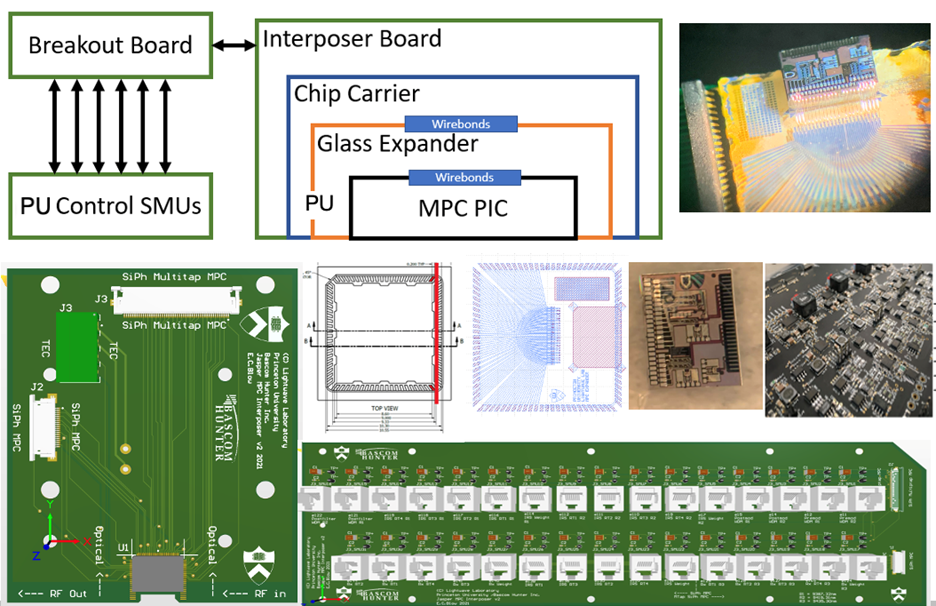
\includegraphics[width=5in]{./Figures/AppendixA/FigAppA01}
\caption{Diagram of packaging approach for silicon microwave photonic canceller}
\label{FigAppA1}
\end{figure}

\section{Fabrication of Glass Expander}
Author and Recipe Developer: Simon Bilodeau

\qquad The fabrication of an expander chip is required to transition from the high density electrical I/O of the PIC to the lower density electrical I/O of a chip carrier. This enables higher density I/O, shorter wirebonds, and multiple rows of wirebonds. Currently, these chips are only utilized passive routing for DC connections. Although, it would be advantageous to surface mount capacitors on this packaging layer for improved RF performance. The following recipe was designed for 4" silica wafer with aluminum traces. Shown in Figure \ref{FigAppA2} below, is an example of a glass expander design used for a microwave photonic canceller. 

\begin{enumerate}
    \item Write the 4" or 5" chrome hard mask \textbf{negative} using a direct write lithography tool. 
    \item Develop, etch chrome, and strip resist in TMAH tank. 
    \item Perform a solvent clean on the wafer with acetone and isopropanol followed by an oxygen plasma clean (5 min, 500 W O2 ashing).
    \item Perform a 5000A aluminum deposition. 
    \item Spin AZ1518 resist (4000 rpm, 40 seconds) followed by a 1 min soft bake at 95°C. 
    \item Expose wafer with standard dose and time for AZ1518.
    \item Develop in AZ 300 MIF for 40s and inspect result under the microscope.
    \item Run a plasma descum (5 min, 200 W O2 ashing) [Recommended but optional].
    \item Aluminum Etch Type A at 50$^{\circ}$C for a few minutes until change is visible.
\end{enumerate}

\qquad This procedure is updated from the recipe presented by the authors in Thomas Ferrier de Lima’s  “Neuromorphic Computing with Silicon Photonics” (2022) \cite{deLimaThesis}. The recipe was modified by change from an aluminum deposition of positive mask and lift-off to aluminum deposition of negative mask and aluminum etch. This transition resulted in a faster process, higher quality traces, and higher yields. 

\begin{figure}[!ht]
\centering
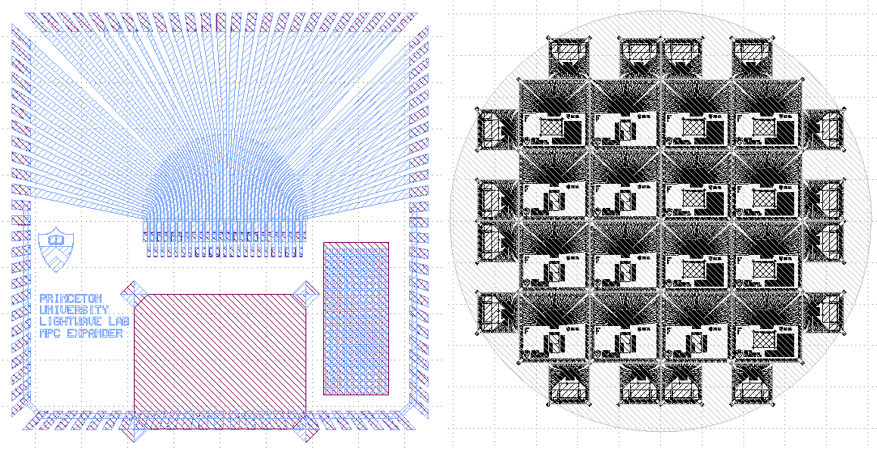
\includegraphics[width=5in]{./Figures/AppendixA/FigAppA02}
\caption{Expander designs for fabricated 4” silica wafer}
\label{FigAppA2}
\end{figure}

\section{ADT Dicing Expander}

\qquad After the customized expander wafer is fabricated within MNFL Cleanroom, the glass or silicon expander wafer must be diced to remove the experiment-specific expander. This process of dicing a 4-inch wafer is standard and requires a few steps, stated below. 

\begin{enumerate}
    \item Mount wafer with the ADT metal ring and 90 $\mu m$ tape.
    \item Measure the height of the tape and confirm 90 $\mu m$.
    \item Flip mounted wafer and apply a second layer of tape to top of wafer. This is done to prevent the expanders from being scratched in the dicing process or afterwards while stored.
    \item Define the appropriate recipe for the ADT Dicing saw.
        \begin{enumerate}
            \item Recipe: Si\_Dice or Glass\_Dice
        \end{enumerate}
    \item Adjust Recipe with the actual height of the tape using the Mitutoyo Height Gauge minus 10 microns and also define the 0 degree and 90 degree dicing index.	
    \item Insert Correct Blade:
        \begin{enumerate}
            \item 2045 Blade for silicon
            \item ADT Resin Blade for glass
        \end{enumerate}
    \item System Init*
    \item Calibrate blade*
    \item Calibrate Y-offset*
    \item Partial cuts plus manual alignment to dice wafer*. On the ADT Dicing, be careful using full wafer cut; There is no confirmation, and the entire wafer will cut after index definition.
\end{enumerate}
*Use Tool Manual for additional detailed instruction.

\begin{figure}[!ht]
\centering
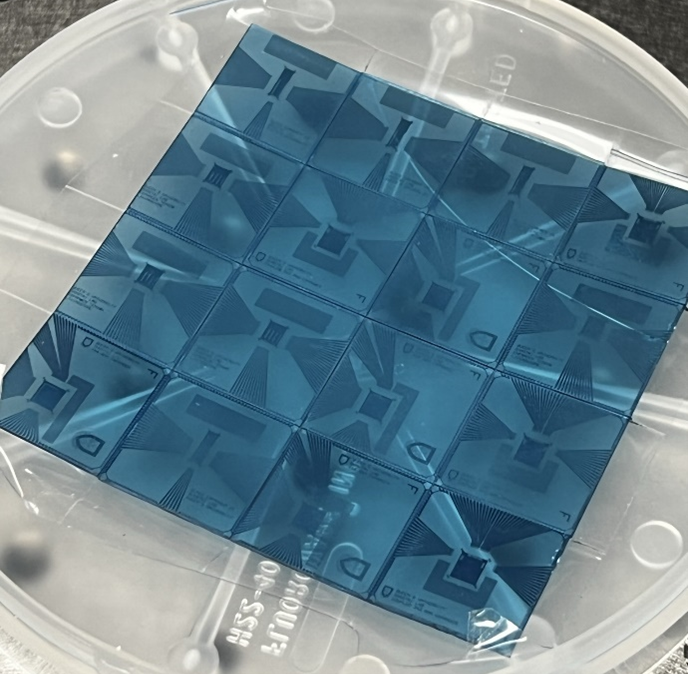
\includegraphics[width=3in]{./Figures/AppendixA/FigAppA03}
\caption{Diced glass expander used for photonic integrated circuit packaging}
\label{FigAppA3}
\end{figure}

\section{Silicon Photonic Integrated Circuit Die Dicing – Z-Cut}

\qquad In integrated photonic prototyping, research groups will leverage multi-project wafer (MPW) runs. The foundry will offer many customers an 8-inch wafer to share, resulting in a user getting 10s of copies of a standardized sized die (commonly 3mm by 8mm). Research groups can utilize this space more effectively by further dividing the chip area into groups of experiments. The division of a single PICs into sub-PICs is highly beneficial for two reasons. Firstly, an increased copy of available chips per experiment, without further dicing of the PIC such as 32 copies of a PIC with 4 experiments would result in 8 copies per experiment. This is due to an inability to package all experiments simultaneously. Secondly, as shown in the figure below, the sub-grouping of experiments significantly increases the available chip parameter for electrical and optical I/O. 

\begin{figure}[!ht]
\centering
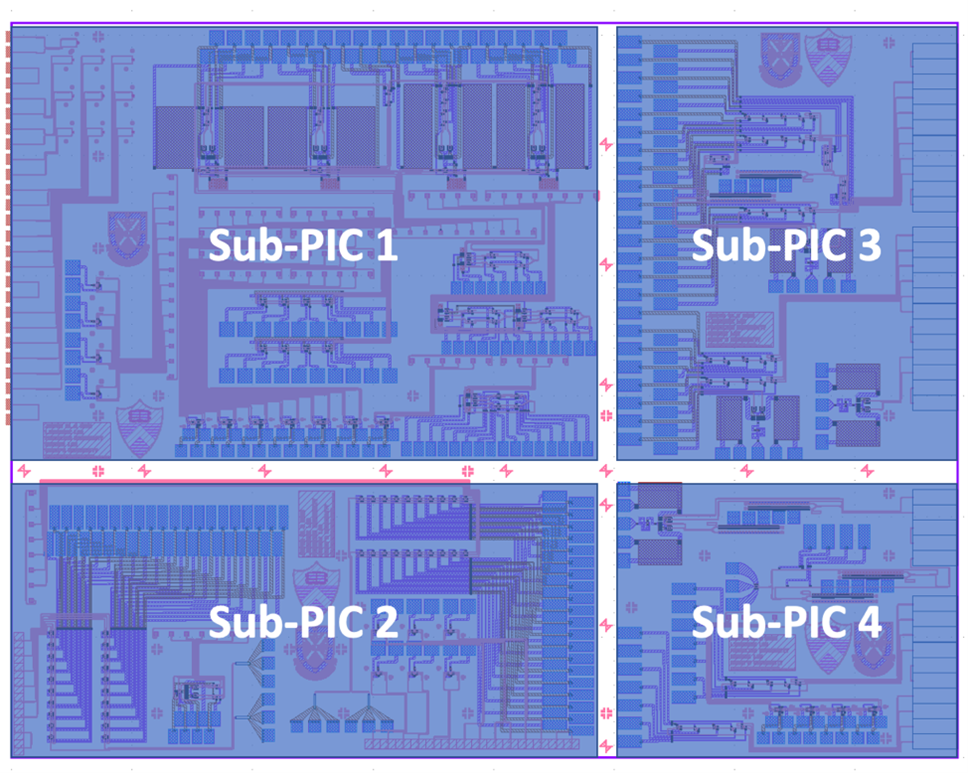
\includegraphics[width=4in]{./Figures/AppendixA/FigAppA04}
\caption{Lightwave Lab’s 6 mm by 10 mm Photonic Integrated Circuit (PIC) sub-grouped into four sub-PICs. The 100 $\mu m$ dicing lanes are indicated by alignment markers.}
\label{FigAppA4}
\end{figure}

\qquad Preforming such a dice on a small sample using a wafer dicing saw requires custom techniques and recipes as to not damage or dislodge the sample. The Z-cut recipe was developed to bring the dicing down in the Z direction over top of the sample. Rather than dicing from the side such as a traditional dicing saw recipe. The recipe is designed to cut with a much slower movement to reduce horizontal forces. For large samples the recipe allows for travel in the positive x-direction (right) after the initial cut is made. 

\qquad This is an updated procedure to the one developed by the authors presented in Thomas Ferrier de Lima’s  “Neuromorphic Computing with Silicon Photonics” (2022)\cite{deLimaThesis}.

\subsection{Carrier Wafer Preparation}
Optional: Prepare a carrier wafer with guidelines to make finding the sample using the ADT significantly easier. 

\begin{enumerate}
    \item Take a relatively clean bulk silicon carrier wafer and use a tex wipe wet with acetone to remove any debris or previous wax from top and back.
    \item Mount the wafer with the tape and metal ring.
    \item Measure the surface of the carrier wafer and set the cutting depth of the recipe to 20 $\mu m$ before the surface of the wafer.
    \item Load the carrier wafer into the ADT dicing saw and define the recipe as the standard Si dicing recipe, e.g. $Si_Test$.
    \item Follow the ADT manual to perform the following 20 $\mu m$ dice.
    \item Avoid dicing too deeply, beyond 20 $\mu m$ can scribe the wafer and encourage breaking along the lattice dislocation line.
    \item Remove sample and clean excess tape residue with acetone.
\end{enumerate}

\begin{figure}[!ht]
\centering
\includegraphics[width=5in]{./Figures/AppendixA/FigAppA05}
\caption[Diagram of guidelines on Si carrier wafer. Example of Si carrier wafer with etched guidelines.]{Diagram of guidelines on Si carrier wafer (left) Example of Si carrier wafer with etched guidelines (right)}
\label{FigAppA5}
\end{figure}

\textbf{Sample Preparation}
\begin{enumerate}
    \item Take a prepared carrier wafer and acetone wipe the wafer. Fold acetone wipe to only clean with a clean side of the wipe. 
    \item Roughly clean back with acetone wipe using the same technique before mounting as carrier wafer will dislodge while dicing if dirty. 
    \item Heat carrier wafer at 165oF (74oC).
    \item Use razor to chisel small shards of crystalline wax from tube
    \item If Z-cutting multiple samples orient them so there is no chance of the dicing blade hitting more than one sample at a time.
\end{enumerate}

\begin{figure}[!ht]
\centering
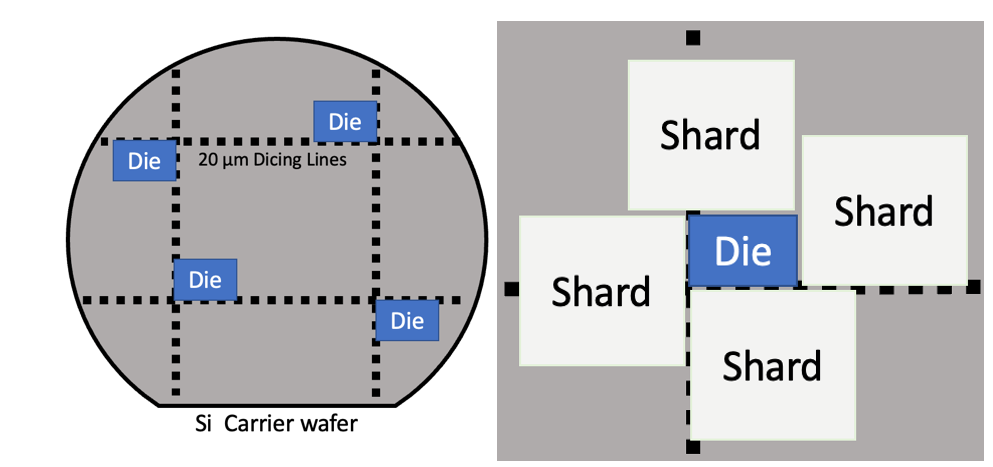
\includegraphics[width=5in]{./Figures/AppendixA/FigAppA06}
\caption[Illustration on how to place multiple samples for Z-cut and how to support a die with space Si or Glass shards.]{Illustration on how to place multiple samples for Z-cut (left) and how to support a die with space Si or Glass shards (right).}
\label{FigAppA6}
\end{figure}

\begin{enumerate}
    \setcounter{enumi}{5}
    \item Put one large shard where the PIC will be located, where all four support shards are located, and the corners where support shards interface with the chip. Place carrier wafer on 80$^{\circ}$C hot plate. Mid-range melting point of 165$^{\circ}$F (74$^{\circ}$C).
\end{enumerate}

\begin{figure}[!ht]
\centering
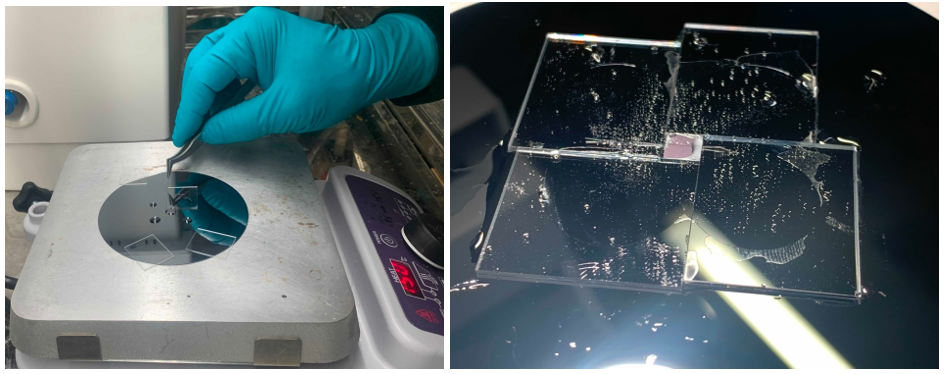
\includegraphics[width=5in]{./Figures/AppendixA/FigAppA07}
\caption[Placing crystalline wax shards where sample and supports are to be located.]{Placing crystalline wax shards where sample and supports should be located (left) Image of mounted sample (right)}
\label{FigAppA7}
\end{figure}

\begin{enumerate}
    \setcounter{enumi}{6}
    \item Ensure chips are loaded onto carrier with same orientation locked into place with 3-4 sides of silicon shards, shown below.
    \begin{enumerate}
        \item If there are edge couplers, you can avoid supporting them with a fourth shard to protect the edge couplers from mechanical damage. There is a risk tradeoff between too poorly supporting the chip or damaging the interface.
    \end{enumerate}
    \item Precisely clean back, 1 wipe per surface of the acetone-soaked Tex wipe to avoid dislodgement.
    \item Measure Z in different places to make sure it’s flat with the Mitutoyo Height Gauge. 
    \begin{enumerate}
        \item Example of Measuring before cut: 
        \begin{enumerate}
            \item Tape height = 120-180 $\mu m$
            \item Tape + Carrier height = 700-800 $\mu m$
            \item Tape + Carrier + Chip = 2500 – 2700 $\mu m$
            \item Cut down to 600$\mu m$ (100$\mu m$ below your carrier height)
        \end{enumerate}
    \end{enumerate}
    \item Roll tape on the carrier without the wafer. 
    \item Slowly apply carrier wafer to tape.
    \begin{enumerate}
        \item Place wafer underneath, making sure there are no gaps. Start with one edge of the wafer and stick the tape gradually and gently with your thumb across the wafer, avoiding bubbles. 
    \end{enumerate}
\end{enumerate}

\textbf{Changes to recipe:}
\begin{enumerate}
    \item Previously used beeswax
    \begin{enumerate}
        \item Problem: beeswax is weaker than crystalline wax.
    \end{enumerate}
    \item Previously used wax shards on top of sample
    \begin{enumerate}
        \item Problem 1: Too little wax sample is not secure, and sample can be dislodged.
        \item Problem 2: Too much wax is hard to see through and therefore hard to align.
        \item Problem 3: Too much wax causes a high wax profile which wears heavily on blade.
        \begin{enumerate}
            \item i.	Previously, height was reduced by using an acetone-soaked wipe Even though successful, there is a need for further reduction. The risk of wax height is due to the 30,000 RPM saw melting the wax on top as cutting and then the wax can get onto the side of blade. 
        \end{enumerate}
    \end{enumerate}
\end{enumerate}

\textbf{Z-cut Dice}
\begin{enumerate}
    \item Load the carrier into the ADT*.
    \item Select the appropriate blade.
    \begin{enumerate}
        \item Blade 2045 for Silicon PICs
        \item 60 $\mu m$ cut width
    \end{enumerate}
    \item Recipe for Z-cut: $ZcutCMOS$ (set cut depth and wafer thickness).
    \item Change recipe to include your calculated cut depth on both cut angles
    \item Decide if you need to increase the cut distance. This may be necessary for dicing larger chips. 
    \item Perform Y-offset.*
    \item Perform partial wafer alignment (skip second angle).*
    \item Partial wafer cut. Access this option via manual, cut, partial. Use animation mode. After selecting it, assuming the wafer alignment is done, proceed with next-next-next-finish-finish.*
    \item After the cut, the ADT tries to unload wafer. Cancel to abort and move to the next cut instead.*
\end{enumerate}

\textbf{Cleaning}
\begin{enumerate}
    \item Heat chip to 80$^{\circ}$C and remove sample with tweezers.
    \item Slide sample into acetone bath for 60 seconds.
    \item Slide onto Tex wipes to clean with Isopropyl Alcohol (IPA).
    \item Repeat cleaning if there is still crystalline wax debris. 
    \item Dry with Nitrogen Gun.
\end{enumerate}
*Use Tool Manual for additional detailed instruction

\begin{figure}[!ht]
\centering
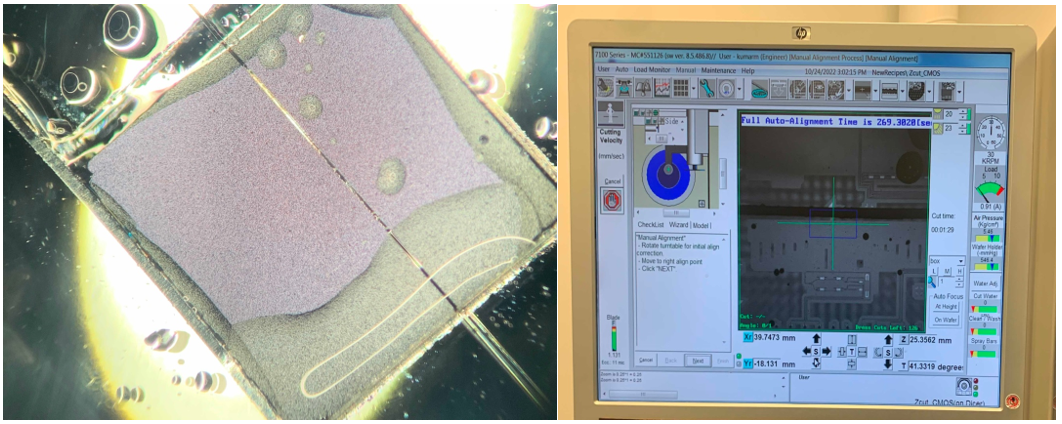
\includegraphics[width=5in]{./Figures/AppendixA/FigAppA08}
\caption[Diced practice sample with improved recipe and ADT dicing saw display after successful z-cut is completed.]{Diced practice sample with improved recipe  (left) and ADT dicing saw display after successful z-cut is completed (right).}
\label{FigAppA8}
\end{figure}

\begin{figure}[!ht]
\centering
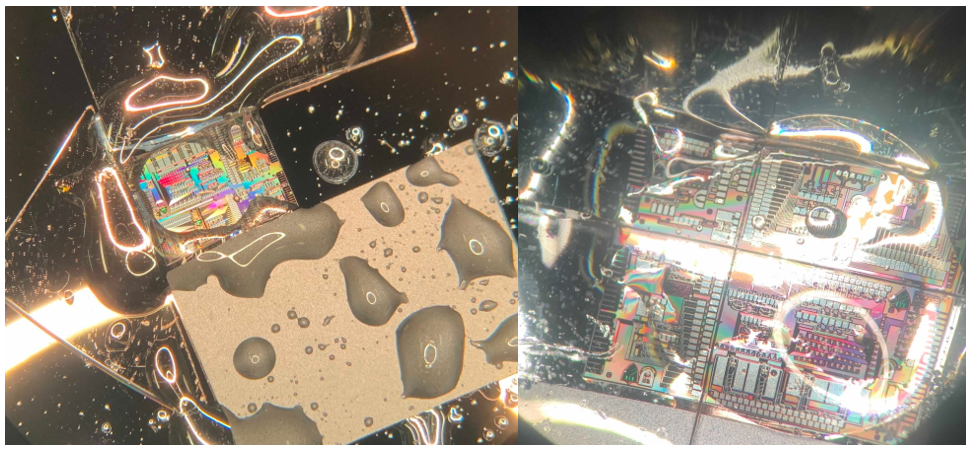
\includegraphics[width=5in]{./Figures/AppendixA/FigAppA09}
\caption[Previously diced samples.]{Previously diced samples. Only covering edges with wax increased risk of sample dislodgement from the carrier (left). Samples with too much wax on the sample caused wear to the blade and was hard to align, even after significant removal with acetone Tex wipe (right). }
\label{FigAppA9}
\end{figure}

\section{Tresky Pick and Place (P\&P)}
\subsection{Direct to chip carrier (Low I/O Count):}
\qquad Direct pick and place (p\&P) to Chip carrier without expander chip. This technique is fast and effective for small-scale experiments with low I/O count (less than 15). The I/O count is limited in this technique because the DC pad array on-chip and the chip carrier have a mismatched pitch. Therefore, the angles generated by the wirebonds will eventually become too great and wirebonds can often short. Additionally, this is only recommended for DC connections due to increased wire bond length relative to packaging with the glass expander or a custom carrier. This increased wire bond length results in a higher inductance which would cause high attenuation if these were used for AC signal. 

\begin{enumerate}
     \item Select DIP package which matches the needs of PIC.
    \item Secure DIP to grated holder with the amber cleanroom electrical tape due to the high melting temperature.
    \item Vacuum metal grated holder to Tresky flip chip bonder main stage. 
    \item Program 28 Pick and Place (P\&P)
    \item Parameters
    \begin{enumerate}
        \item Force:
        \begin{enumerate}
            \item Pick: 30g
            \item Place: 250g
        \end{enumerate}
        \item Time:
        \begin{enumerate}
            \item Pick: 250 ms
            \item Place: 250 ms
            \item Scrub: 0 ms
            \item Del. S: 0 ms            
        \end{enumerate}
        \item Height:
        \begin{enumerate}
            \item Program dynamically due to height of dip and chip
        \end{enumerate}
        \item Puff time: disable
        \item Puff offset: disable
        \item Speed:
        \begin{enumerate}
            \item Pick down: 1 mm/s
            \item Pick up: 5 mm/s 
            \item Place down: 1 mm/s (as slow as possible)
            \item Clearance: 40 mm/s
        \end{enumerate}
        \item QH Place force (applies force while heating and curing epoxy)
    \end{enumerate}
    \item Define heat profile based on silver epoxy specification sheet. 
    \begin{enumerate}
        \item Using H20E EPO-TEK Silver conductive epoxy Product No. 16014
        \item 120$^{/circ}$C for 15 min.
        \item Make sure TEC unit is enabled or Tresky will stall out and require reboot.
    \end{enumerate}
    \item Define height parameters using microscope and shortcut Tresky buttons.
    \item Dry run with dummy Sample, Pick and Place with Quick Heat off to check heights and forces but not have to wait for heating cycling.
    \item Remove metal grated holder with dip package from Tresky.
    \item Apply blue tape to entire surface of dip and cut a rectangle hole approximately the same size as the chip being packaged .
    \item Mix the two-part epoxy on a glass slide and using a small cotton swab apply a thin layer over the blue tape.
    \item Remove the blue tape and left behind is the square epoxy.
    \item Remount the metal grating holder to the Tresky flip chip bonding
    \item Turn Quick Heat On and run the Pick and Place programming, aligning, and then curing the sliver epoxy.
    \begin{enumerate}
        \item Align the sample to the DIP package with reflection of the samples. Aim for the midpoint between the nozzle and the reflection. This point is where the chip edge will meet the chip.
    \end{enumerate}
\end{enumerate}


\begin{figure}[!ht]
\centering
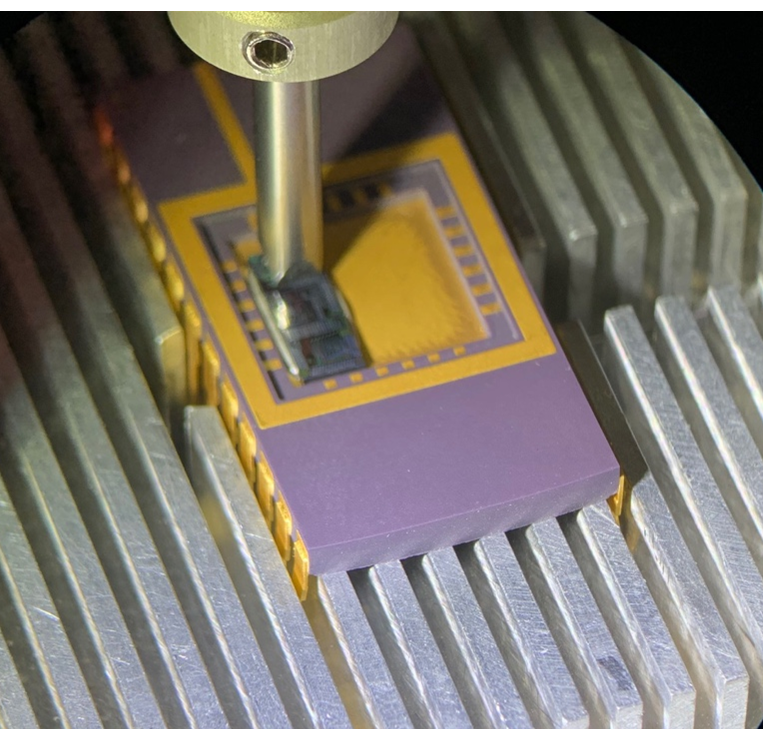
\includegraphics[width=3.5in]{./Figures/AppendixA/FigAppA10}
\caption{DIP carrier mounted to metal grating holder. Tape corners for added stability}
\label{FigAppA10}
\end{figure}

\begin{figure}[!ht]
\centering
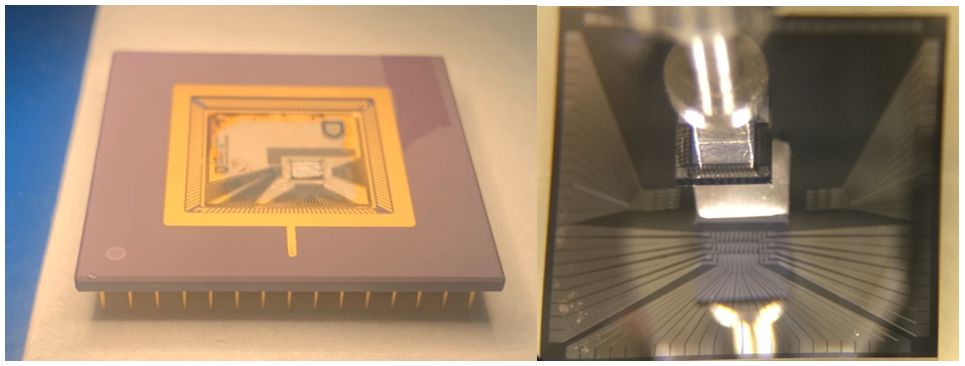
\includegraphics[width=5in]{./Figures/AppendixA/FigAppA11}
\caption[Pick and Place examples.]{Sample with silver epoxy applied (left) and sample with PIC being placed by Tresky P\&P (right)}
\label{FigAppA11}
\end{figure}

\begin{figure}[!ht]
\centering
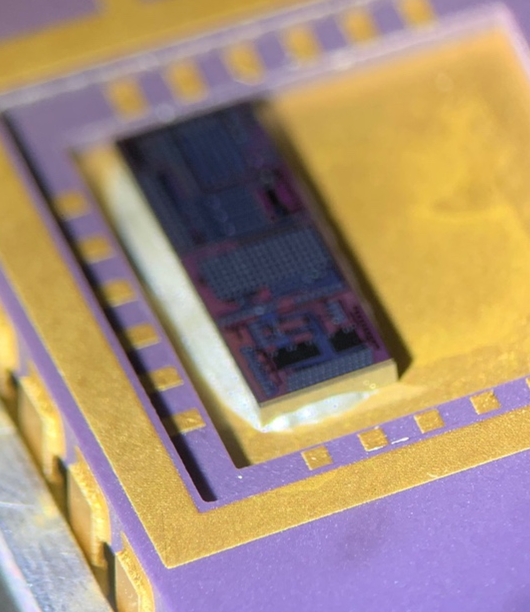
\includegraphics[width=3.5in]{./Figures/AppendixA/FigAppA12}
\caption{PIC epoxied directly to DIP chip carrier.}
\label{FigAppA12}
\end{figure}

\subsection{PIC, Expander, Chip Carrier stack (High I/O Count):}

\begin{figure}[!ht]
\centering
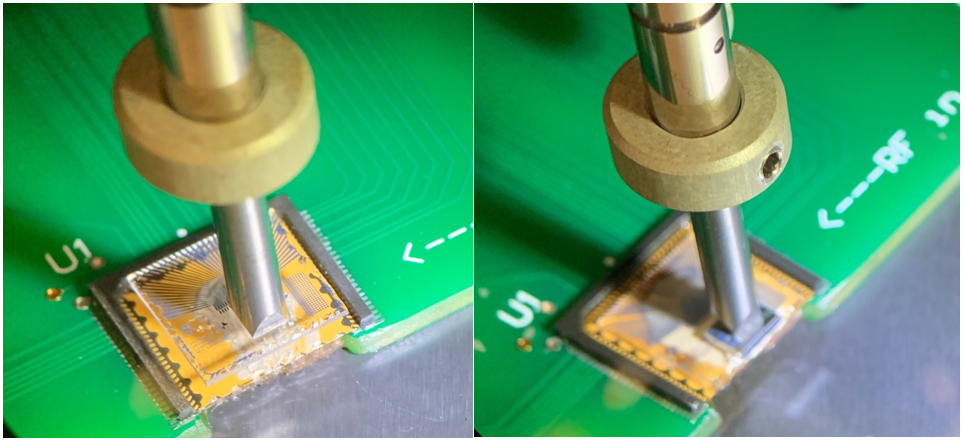
\includegraphics[width=5in]{./Figures/AppendixA/FigAppA13}
\caption[Glass expander being placed and epoxied to custom chip carrier. PIC being placed and epoxied to glass expander.]{Glass expander being placed and epoxied to custom chip carrier (left), PIC being placed and epoxied to glass expander (right).}
\label{FigAppA13}
\end{figure}

\begin{figure}[!ht]
\centering
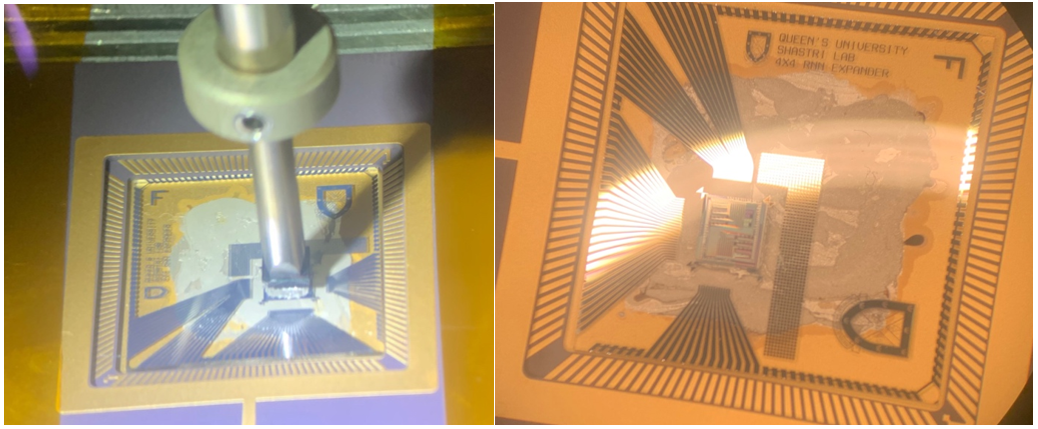
\includegraphics[width=5in]{./Figures/AppendixA/FigAppA14}
\caption{Chip Carrier, Glass Expander, PIC epoxying procedure.}
\label{FigAppA14}
\end{figure}

\textbf{Discussion:}
\qquad There is a risk trade-off between the soldering chip carrier to the PCB board before wirebonding or afterwards. My recommendation is to bond first for small I/O prototyping and to solder to first for large scale I/O.

\qquad If one was to first solder the chip carrier, there would be no risk of damaging the bonds while soldering. This process requires heat and mechanical manipulation, which could result in accidental damage to the bonds. There would also be the risk of damaging the FR4 PCB board during the curing process. Upon detailed observation, discoloration and smoking took place initially but stabilized after 15 seconds. Neither damage nor degradation of performance was observed. The primary problem with soldering first on the small I/O DIP packages is twofold. Firstly, it is difficult to achieve the security and planarization required for wirebonding in a standard through-hole or pluggable standardized chip carrier package. Additionally, not only must the carrier be planar, but also the board must be. If the board is planned significantly in advance and there are mounting holds which match the Tresky and Questar mounts to stabilize the board and chip carrier, soldering first is recommended. The sample must be absolutely secure and planar or the bonding yield will be very poor ($< 80\%$). For prototyping small I/O counts, using the metal grating and soldering afterwards is an easier and more flexible approach. For large I/O counts, plan ahead and incorporate mounting holds and solder first. 

\section{Questar Automatic Wedge Wire Bonder}
\qquad Wire bonding is a tedious but critical part of the packaging procedure. The PICs, glass expanders, and chip carriers were electrically interfaced with 25 $\mu m$ wedge wire bonds. The challenge within this research was two-fold. Firstly, the authors needed to achieve a high yield to successfully bond 300+ wire bonds without failure. This was due to a high number of electrical I/O and small pad sizes on the PIC which only allowed for one bonding attempt. Second, given the limited chip perimeter, the authors developed a three-row recipe to three-fold increase the amount of possible electrical I/O. There was a critical need to scale the size of the photonic neural network. The yield of the wire bonding is dependent on:

\begin{enumerate}
    \item Requirement: Planarization of the PIC and glass expander.
    \begin{enumerate}
        \item Solution: the use of the Tresky for Pick and Place.
    \end{enumerate}
    \item Requirement: Firm mounting of sample to Questar.
    \begin{enumerate}
        \item Solution: Design custom PCBs with drill holes matching the mounting of the Questar.
    \end{enumerate}
    \item Requirement: Parallel Wirebonds
    \begin{enumerate}
        \item Solution: Design glass expanders in Princeton Cleanroom with matching pad arrays to that which are on the PIC.
    \end{enumerate}
    \item Requirement: Clean surfaces and quality metalization. 
    \begin{enumerate}
        \item Solution: Cleaning pads before bonding and optimized glass expander recipe (see Appendix A3)
    \end{enumerate}
\end{enumerate}

\qquad By applying these solutions, the authors developed a packaging recipe with a percent yield of more than 99\%. To achieve the three rows of wire bonds for the high density photonic neural network, the authors fabricated dummy replicas of the PICs and optimized the physical parameters of the wire bonds by trial and error. The result of the recipe development is stored in memory on the Tresky and provided in the Table 1 below. Lastly, the authors determined the inclusion of a pad array “graveyard” on the glass expander was critically important. These additional free pads can be used for calibration, ensuring proper bonding operation after a failed bond, and removal of the wire bond tail caused by re-threading. 

\textbf{Sample and Equipment Preparation:}

\begin{enumerate}
    \item Clean pads with acetone, if possible, and/or at least IPA to remove any potential organic debris
    \item Firmly and securely mount the sample to the Questar Wire Bonder.
    \begin{enumerate}
        \item This can be done with metal grates if a small through-hole I/O chip carrier is used.
        \item Ideally, the designer planned for wire bonding and the sample is on a custom PCB with 4 holes created which match the mounting brackets of the Questar.
        \begin{enumerate}
            \item Screw hole: 9 AWG (2.9 metric)
            \item Horizontal separation: 4 cm
            \item Vertical separation: 4.5 cm
        \end{enumerate}
    \end{enumerate}
    \item Unthread the wire from the wedge tool and calibrate for x-y position and ultrasonics, following the manual.
    \begin{enumerate}
        \item This calibration should be done on the pad array graveyard on glass expander.
    \end{enumerate}
    \item Select the PIC row or expander to chip carrier recipe. 
    \item Begin bonding in accordance with the equipment manual. 
    \item Check pad footprint width to ensure it meets the 1.5x wire bond width which ensures appropriate levels.
    \begin{enumerate}
        \item If too wide lower ultrasonic power, if too narrow increase ultrasonic power
    \end{enumerate}
\end{enumerate}

\begin{figure}[!ht]
\centering
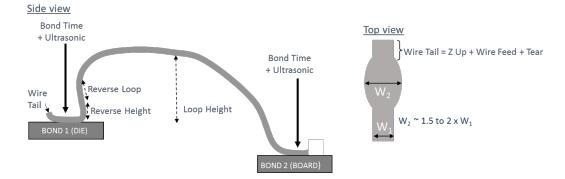
\includegraphics[width=5in]{./Figures/AppendixA/FigAppA15.png}
\caption{Wedge wire bond parameter definitions and expected range. Source: Princeton MNFL  }
\label{FigAppA15}
\end{figure}

\begin{figure}[!ht]
\centering
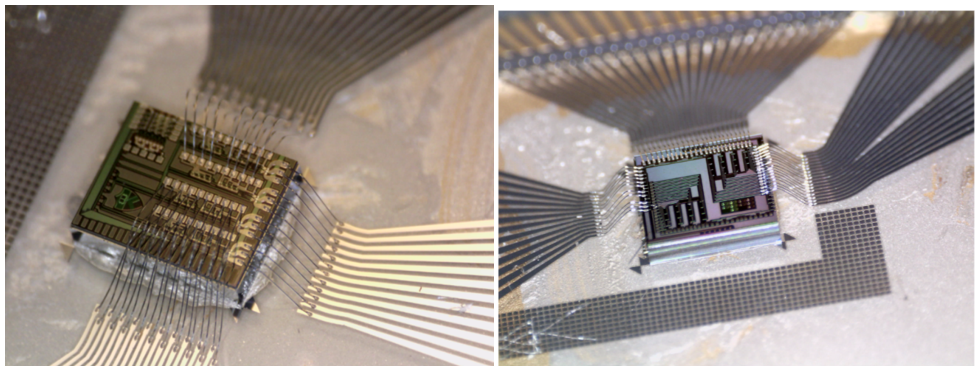
\includegraphics[width=5in]{./Figures/AppendixA/FigAppA16.png}
\caption{Two fully packaged photonic integrated circuits demonstrating high density electrical I/O. Optical I/O is not shown. }
\label{FigAppA16}
\end{figure}


\begin{table}[!ht]
\caption[Questar Wire bond Recipes: Expander to Chip Carrier]{\textbf{Questar Wire bond Recipes: Expander to Chip Carrier}}
\centering
\begin{tabular}{|c||c|}
\hline
Parameter & Value for glass expander \\ \hhline{|=|=|}
Bond 1 CV Height & 35 mils   \\ \hline
Bond 1 Overtravel & 1 mils   \\ \hline
Bond 1 Bond Time & 60 ms    \\ \hline
Bond 1 Ultrasonics & 50 power   \\ \hline
Loop Reverse Height & 10 mils  \\ \hline 
Loop Reverse Loop & 10 mils  \\ \hline
Loop Height & 35 mils \\ \hline
Bond 2 CV Height & 35 mils   \\ \hline
Bond 2 Overtravel & 1 mils   \\ \hline
Bond 2 Bond Time & 55 ms   \\ \hline
Bond 2 Ultrasonics & 54   \\ \hline
Z up & 2.1 mils \\ \hline
Wire Feed & 2.8 mils \\ \hline
tear & 1.5 mils  \\ \hline
\end{tabular}
\end{table}

\begin{table}[!ht]
\caption[Questar Wire bond Recipes: PIC Row 1]{\textbf{Questar Wire bond Recipes: PIC Row 1}}
\centering
\begin{tabular}{|c||c||c|}
\hline
Parameter & Value for AMF & Value for IME \\ \hhline{|=|=|=|}
Bond 1 CV Height & 35 mils & 35 mils \\ \hline
Bond 1 Overtravel & 1 mils & 1 mils \\ \hline
Bond 1 Bond Time & 50 ms & 50 ms \\ \hline
Bond 1 Ultrasonics & 49 power & 50 power \\ \hline
Loop Reverse Height & 10 mils & 10 mils \\ \hline 
Loop Reverse Loop & 10 mils & 10 mils \\ \hline
Loop Height & 36 mils & 36 mils \\ \hline
Bond 2 CV Height & 35 mils & 35 mils \\ \hline
Bond 2 Overtravel &  1.2 mils & 1.2 mils \\ \hline
Bond 2 Bond Time & 60 ms & 60 ms \\ \hline
Bond 2 Ultrasonics & 55 power & 55 power \\ \hline
Z up & 2.6 mils & 2.6 mils \\ \hline
Wire Feed & 2.6 mils & 2.6 mils \\ \hline
tear & 1.5 mils & 1.5 mils  \\ \hline
\end{tabular}
\end{table}

\begin{table}[!ht]
\caption[Questar Wire bond Recipes: PIC Row 2]{\textbf{Questar Wire bond Recipes: PIC Row 2}}
\centering
\begin{tabular}{|c||c||c|}
\hline
Parameter & Value for AMF & Value for IME \\ \hhline{|=|=|=|}
Bond 1 CV Height & 35 mils & 35 mils \\ \hline
Bond 1 Overtravel &  1 mils & 1 mil \\ \hline
Bond 1 Bond Time & 62 ms & 62 ms \\ \hline
Bond 1 Ultrasonics & 49 power  & 56 Power \\ \hline
Loop Reverse Height & 12 mils & 12 mils \\ \hline 
Loop Reverse Loop & 20 mils & 20 mils \\ \hline
Loop Height & 40 mils & 40 mils \\ \hline
Bond 2 CV Height & 35 mils  & 35 mils \\ \hline
Bond 2 Overtravel & 1.2 mils & 1.2 mils \\ \hline
Bond 2 Bond Time &  65 ms &  65 ms\\ \hline
Bond 2 Ultrasonics & 55 power  &  59 power \\ \hline
Z up & 2.3 mils & 2.3 mils \\ \hline
Wire Feed & 3 mils & 3.2 mils \\ \hline
tear &  1.5 mils & 1.5 mils \\  \hline
\end{tabular}
\end{table}

\begin{table}[!ht]
\caption[Questar Wire bond Recipes: PIC Row 3]{\textbf{Questar Wire bond Recipes: PIC Row 3}}
\centering
\begin{tabular}{|c||c||c|}
\hline
Parameter & Value for AMF & Value for IME \\ \hhline{|=|=|=|}
Bond 1 CV Height & 35 mils & 35 mils \\ \hline
Bond 1 Overtravel &  1 mil &  1 mil \\ \hline
Bond 1 Bond Time & 60 ms & 60 ms\\ \hline
Bond 1 Ultrasonics &  49 power & 40 power \\ \hline
Loop Reverse Height & 35 mils & 35 mils \\ \hline 
Loop Reverse Loop & 33 mils & 33 mils \\ \hline
Loop Height & 58 mils & 58 mils \\ \hline
Bond 2 CV Height &  35 mils  & 35 mils \\ \hline
Bond 2 Overtravel &  1 mil &  1 mils \\ \hline
Bond 2 Bond Time &  63 ms &  63 ms \\ \hline
Bond 2 Ultrasonics &  55 power &  40 power \\ \hline
Z up &  2.3 mils & 2.3 mils \\ \hline
Wire Feed & 3 mils & 3 mils \\ \hline
tear & 1.5  mils & 1.5 mils \\ \hline
\end{tabular}
\end{table}

\begin{table}[!ht]
\caption[Questar Wire bond Recipes: Static Parameters]{\textbf{Questar Wire bond Recipes: Static Parameters}}
\centering
\begin{tabular}{|c||c||c|}
\hline
Static Parameters & Value for AMF & Value for IME \\ \hhline{|=|=|=|}
& Expander to Chip Carrier & \\ \hline
Bond 1 and 2 CV Height &  35 mils &  35 mils \\ \hline
Bond 1 and 2 Contact Velocity  & 100 mils/sec  & 100 mils/sec \\ \hline
Loop Stretch & 0 mils  & 0 mils \\ \hline
Rise to Loop & 0 mils  &  0 mils \\ \hline
Clamp Close & CV Height 2  & CV Height 2 \\ \hline
Reset Height & 35 mils & 35 mils \\ \hline
\end{tabular}
\end{table}

\section{Acknowledgements}
\qquad The authors of these packaging procedures would like to thank and acknowledge the Princeton MNFL cleanroom and staff. Specifically, Bert G. Harrop for his guidance and expertise in developing the recipes presented here. The authors would also like to thank Zuzanna Lewicka for authoring the packaging equipment manuals referenced within this appendix
